\documentclass[12pt, a4paper]{article}

% ---------- Paket ----------
\usepackage[utf8]{inputenc}
\usepackage[T1]{fontenc}
\usepackage[indonesian]{babel}
\usepackage{amsmath, amssymb}
\usepackage{graphicx}
\usepackage{caption}
\usepackage{subcaption}
\usepackage{float}
\usepackage{hyperref}
\usepackage{booktabs}
\usepackage{array}
\usepackage{longtable}
\usepackage[table]{xcolor}
\usepackage{listings}
\usepackage{parskip}
\usepackage[a4paper, top=2.5cm, bottom=2.5cm, left=3cm, right=3cm]{geometry}

% ---------- Listing Java ----------
\definecolor{codegray}{rgb}{0.5,0.5,0.5}
\definecolor{codeblue}{rgb}{0.13,0.29,0.53}
\definecolor{codegreen}{rgb}{0.0,0.4,0.0}
\definecolor{codepurple}{rgb}{0.55,0.0,0.55}
\lstdefinestyle{javastyle}{
    language=Java,
    basicstyle=\small\ttfamily,
    keywordstyle=\color{codeblue}\bfseries,
    commentstyle=\color{codegreen}\itshape,
    stringstyle=\color{codepurple},
    numberstyle=\tiny\color{codegray},
    breaklines=true,
    frame=single,
    numbers=left,
    numbersep=5pt,
    showstringspaces=false,
    tabsize=4,
}
\lstset{style=javastyle}

% Gambar menggunakan path eksplisit dari direktori .tex ini (public/...)

% ---------- Hyperref ----------
\hypersetup{
    colorlinks=true,
    linkcolor=black,
    urlcolor=blue,
}

% ---------- Judul ----------
\title{
    \textbf{Battlecode 2025 Postmortem} \\[0.4cm]
    \large IF2211 Strategi Algoritma --- STIMA-BATTLE 2026
}
\author{
    Athilla Zaidan Zidna Fann (13524068) \\
    Kevin Wirya Valerian (13524019) \\
    Muhammad Aufar Rizqi Kusuma (13524061) \\[0.2cm]
    \textit{Kelompok Jambi X Bekasi}
}
\date{Semester II 2025/2026}

% ================================================================
\begin{document}
\maketitle
\tableofcontents
\newpage

% ================================================================
\section{Pendahuluan}

Kami adalah kelompok \textbf{Jambi X Bekasi}, terdiri dari tiga mahasiswa Teknik
Informatika ITB angkatan 2024 yang berkompetisi dalam \textit{STIMA-BATTLE 2026},
turnamen berbasis Battlecode 2025 yang diselenggarakan dalam rangka Tugas Besar 1
mata kuliah IF2211 Strategi Algoritma.

Ini merupakan pengalaman pertama kami berpartisipasi dalam kompetisi berbasis
Battlecode. Kami mulai membangun bot dari nol tanpa referensi kode eksternal,
mengandalkan spesifikasi permainan resmi dan diskusi internal kelompok. Pendekatan
yang kami pilih adalah \textit{greedy}: setiap unit membuat keputusan lokal-optimal
pada setiap giliran berdasarkan kondisi yang dapat diobservasi saat itu.

Bot final kami tersimpan pada paket \texttt{main\_bot} di repositori
\textit{greedy\-conqueror}. Selain \texttt{main\_bot}, kami juga mengembangkan dua
varian eksperimental --- \texttt{alternative\_\allowbreak bots\_1} (strategi ofensif
agresif) dan \texttt{alternative\_\allowbreak bots\_2} (maksimisasi cakupan) ---
namun \texttt{main\_bot} adalah yang kami gunakan pada seluruh pertandingan turnamen.

Dalam turnamen, kami berhasil memenangkan tiga babak pertama dengan skor 2-0
(termasuk satu babak sebagai tim perak) sebelum kalah pada babak keempat dengan
skor 1-2.

% ================================================================
\section{Gambaran Umum Permainan}

Battlecode 2025 adalah permainan strategi real-time berbasis giliran di mana dua
tim saling bersaing untuk menguasai peta berukuran hingga $60 \times 60$ petak.
Setiap tim memiliki beberapa jenis unit dan menara.

\subsection*{Unit dan Menara}

\begin{itemize}
    \item \textbf{Paint Tower} (\textit{Menara Cat}): Menghasilkan cat sebagai
          sumber daya utama. Tanpa cat, unit tidak dapat bergerak maupun bertindak
          secara normal.
    \item \textbf{Money Tower} (\textit{Menara Uang}): Menghasilkan \textit{chips}
          yang digunakan untuk membangun menara dan unit.
    \item \textbf{Defense Tower} (\textit{Menara Pertahanan}): Memiliki kerusakan
          tertinggi dan menghasilkan \textit{chips} saat menyerang unit musuh.
    \item \textbf{Soldier} (\textit{Tentara}): Unit serbaguna --- dapat mengecat
          petak, menyerang menara musuh, dan membangun menara atau SRP.
    \item \textbf{Splasher} (\textit{Pemercik}): Melakukan serangan cat AOE
          (\textit{area of effect}) pada area $3\times3$ di pusat sasaran ditambah
          empat petak kardinal di jarak $\sqrt{4}$, efektif untuk meningkatkan
          cakupan dengan cepat.
    \item \textbf{Mopper} (\textit{Pembersih}): Menghapus cat musuh dan dapat
          melakukan \textit{mop swing} untuk membersihkan area $2\times2$.
\end{itemize}

\subsection*{Sistem Cat dan Ekonomi}

Setiap unit memiliki HP dan level cat individual. Level cat di bawah 50\%
memperlambat gerakan dan aksi, sedangkan level nol mencegah semua aksi dan
menyebabkan penurunan HP secara bertahap. Unit kehilangan cat saat berada di
petak netral atau cat musuh, mendorong strategi pengendalian wilayah.
\textit{Chips} dibagi bersama oleh seluruh tim.

\subsection*{Pola Menara dan SRP}

Unit dapat membangun menara dengan mengecat pola $5\times5$ di sekitar reruntuhan
(\textit{ruin}) yang tersedia di peta. Biaya membangun menara adalah 200
\textit{chips}.

\textit{Special Resource Patterns} (SRP) adalah pola cat $5\times5$ khusus yang,
setelah diaktifkan selama 50 ronde, memberikan \textit{boost} produksi sumber daya.
Beberapa SRP dapat aktif secara bersamaan dan tumpang-tindih. Posisi pusat SRP yang
optimal memenuhi kondisi \textit{tilability}, yaitu $(x \bmod 4, y \bmod 4) = (2, 2)$.

\subsection*{Kondisi Menang}

Tim yang berhasil menguasai (mengecat dengan warna tim sendiri) lebih dari
\textbf{70\%} dari seluruh petak yang dapat dicat pada peta dinyatakan menang.
Apabila tidak ada tim yang mencapai 70\% dalam 2000 ronde, tim dengan persentase
cakupan tertinggi dinyatakan menang.

% ================================================================
\section{Detail Implementasi Bot}

Bot final kami (\texttt{main\_bot}) dirancang dengan prinsip \textbf{greedy lokal}:
setiap unit hanya menggunakan informasi yang dapat diobservasi dalam radius
penginderaannya untuk membuat keputusan terbaik pada setiap giliran. Tidak ada
pencarian \textit{minimax}, tidak ada model lawan, dan tidak ada koordinasi global
yang eksplisit. Setiap unit bertindak secara independen.

\subsection{Arsitektur Modular}

Bot terdiri dari lima kelas kontroler unit (satu per jenis) ditambah dua kelas
pendukung:

\begin{center}
\begin{tabular}{lp{9cm}}
\toprule
\textbf{Kelas} & \textbf{Peran} \\
\midrule
\texttt{RobotPlayer}  & Titik masuk utama; mendelegasikan ke kontroler berdasarkan tipe \\
\texttt{SoldierBot}   & Pembangun menara, penyerang, pembangun SRP \\
\texttt{TowerBot}     & Pemroduksi unit, penyerang, penyiar informasi \\
\texttt{SplasherBot}  & Percepatan cakupan berbasis AOE \\
\texttt{MopperBot}    & Pembersih cat musuh, dukungan unit \\
\texttt{Nav}          & Navigasi: \textit{fuzzy move} + BugNav + anti-osilasi \\
\texttt{Messaging}    & Komunikasi bit-packed 32-bit antar-unit \\
\bottomrule
\end{tabular}
\end{center}

\subsection{SoldierBot --- Unit Inti}

Soldier adalah unit paling penting dalam strategi kami. Ia mengimplementasikan
\textit{greedy state machine} dengan lima status:

\begin{center}
\begin{tabular}{ll}
\toprule
\textbf{Status} & \textbf{Kondisi Masuk} \\
\midrule
\texttt{EXPLORE}     & Default; penjelajahan frontier \\
\texttt{REFILL}      & Level cat $< 10\%$ dan ada menara terdekat \\
\texttt{COMBAT}      & Terlihat menara musuh, HP $> 40$, cat $> 30\%$ \\
\texttt{BUILD\_TOWER} & Ditemukan reruntuhan kosong, \textit{chips} $\geq 200$ \\
\texttt{BUILD\_SRP}  & Jumlah menara $\geq 3$, ada \textit{paint tower}, dan \textit{chips} $\geq 100$ \\
\bottomrule
\end{tabular}
\end{center}

\noindent Keputusan status dibuat setiap giliran melalui fungsi \texttt{greedyDecide()}:

\begin{lstlisting}[caption={Fungsi greedy decision SoldierBot (disederhanakan)}]
private static State greedyDecide(RobotController rc, MapLocation me,
        MapInfo[] nearby, RobotInfo[] allies, RobotInfo[] enemies)
        throws GameActionException {

    double paintRatio = (double) rc.getPaint() / rc.getType().paintCapacity;

    // 1. Prioritas: Isi ulang cat jika hampir habis
    if ((state != State.REFILL && paintRatio < 0.10)
     || (state == State.REFILL && paintRatio < 0.50)) {
        MapLocation pt = findVisibleTowerLoc(allies);
        if (pt == null) pt = Messaging.nearestRefillTower(me);
        if (pt != null && me.distanceSquaredTo(pt) <= 100)
            return State.REFILL;
    }

    // 2. Serang menara musuh jika cukup sehat dan bercat
    RobotInfo enemyTower = Nav.nearestEnemyTower(enemies);
    if (enemyTower != null && rc.getHealth() > 40 && paintRatio > 0.30)
        return State.COMBAT;

    // 3. Bangun menara jika ada reruntuhan dan chips cukup
    bestRuin = findBestRuin(rc, me, nearby, allies);
    if (bestRuin != null && rc.getChips() >= 200)
        return State.BUILD_TOWER;

    // 4. Bangun SRP jika ekonomi stabil
    if (Messaging.towerCount >= 3 && Messaging.countPaintTowers() > 0
        && enemies.length == 0 && rc.getChips() >= 100) {
        bestSRP = findBestSRP(rc, me);
        if (bestSRP != null) return State.BUILD_SRP;
    }

    return State.EXPLORE;
}
\end{lstlisting}

\subsubsection*{Pemilihan Tipe Menara}

Soldier memutuskan tipe menara secara greedy berdasarkan komposisi menara saat ini:
\begin{itemize}
    \item Jika ada musuh dalam radius 6 petak dari reruntuhan dan jumlah
          \textit{defense tower} $< 3$: bangun \textit{defense tower}.
    \item Jika belum ada \textit{paint tower}: bangun \textit{paint tower}.
    \item Jika jumlah \textit{money tower} $\leq$ jumlah \textit{paint tower}: bangun
          \textit{money tower}.
    \item Selain itu: bangun \textit{paint tower}.
\end{itemize}

\subsubsection*{Seleksi Reruntuhan Terbaik}

Fungsi \texttt{findBestRuin()} mengevaluasi setiap reruntuhan yang terlihat dengan
skor:
\[
    \text{skor} = 3 \cdot |\text{petak benar}| - 2 \cdot |\text{petak kurang}| - \frac{d^2}{4}
\]
di mana $d^2$ adalah jarak kuadrat dari posisi Soldier ke reruntuhan. Reruntuhan
dengan cat musuh $> 25\%$ dari total petak diabaikan. Reruntuhan yang sudah
ditangani oleh $\geq 3$ Soldier lain juga dilewati untuk menghindari penumpukan.

\subsubsection*{Mark-Based Painting}

Untuk mengecat pola menara dan SRP, kami menggunakan sistem berbasis \textit{mark}
(\texttt{getMark()}). Soldier pertama kali menandai (\textit{mark}) pola pada grid,
kemudian semua Soldier yang lewat dapat mengecat petak yang \textit{mark}-nya tidak
sesuai dengan cat aktual --- tanpa perlu hard-code posisi relatif setiap petak.

\subsection{TowerBot --- Penghasil dan Penyiar}

Menara bertugas sebagai produsen unit, penyerang musuh terdekat, dan penyiar
informasi jaringan menara.

\subsubsection*{Strategi Spawn Bertahap}

Komposisi unit yang di-\textit{spawn} disesuaikan dengan fase permainan:

\begin{center}
\begin{tabular}{clccc}
\toprule
\textbf{Fase} & \textbf{Ronde} & \textbf{Soldier} & \textbf{Splasher} & \textbf{Mopper} \\
\midrule
Awal   & $< 150$    & 4 & 0 & 1 \\
Tengah & $150$--$400$ & 2 & 2 & 1 \\
Akhir  & $> 400$    & 1 & 2 & 1 \\
\bottomrule
\end{tabular}
\end{center}

Pada fase awal, Soldier diprioritaskan untuk membangun jaringan menara. Pada fase
tengah dan akhir, Splasher diperbanyak untuk mempercepat cakupan wilayah.

\subsubsection*{Serangan Prioritas}

Menara menyerang dengan prioritas: Soldier musuh terlebih dahulu (karena ancaman
terbesar terhadap jaringan menara), kemudian unit dengan HP terendah.

\subsubsection*{Upgrade Menara}

Menara di-\textit{upgrade} secara konservatif:
\begin{itemize}
    \item Level 1 $\to$ 2: setelah ronde 100, memiliki $\geq 3$ menara, dan
          \textit{chips} $\geq 3000$.
    \item Level 2 $\to$ 3: setelah ronde 400, \textit{chips} $\geq 5500$.
\end{itemize}

\subsection{SplasherBot --- Percepatan Cakupan}

Splasher berfokus pada memperluas cakupan cat dengan serangan AOE. Ia tidak
mencoba merusak menara musuh secara langsung.

\subsubsection*{Penentuan Target Splash}

Setiap kandidat lokasi splash dievaluasi dengan nilai:
\[
    v = \sum_{\text{inner}} w_{\text{inner}}(t) + \sum_{\text{outer}} w_{\text{outer}}(t)
\]
di mana area inner adalah $3\times3$ di sekitar pusat (bobot: +4 untuk cat musuh,
+2 untuk petak kosong) dan area outer adalah empat petak kardinal di jarak $d^2=4$
(bobot: +1 untuk petak kosong saja). Target dengan $v \geq 3$ dipilih.

Splasher tidak akan menyerang lokasi yang akan mengenai menara musuh secara tidak
sengaja (karena akan mengaktifkan serangan balasan).

\subsubsection*{Navigasi Splasher}

Splasher mencari \textit{cluster} petak yang dapat dicat (kosong atau cat musuh)
dan bergerak ke arahnya. Jika tidak ada cluster, ia menjelajahi peta menggunakan
BugNav dengan arah yang ditentukan oleh \textit{prime scatter}:
\[
    \text{dir} = (\text{myID} \times 37 + \lfloor \text{ronde}/30 \rfloor) \bmod 8
\]
Rumus ini mendistribusikan Splasher ke berbagai arah dan memperbarui arah secara
berkala untuk mencegah penumpukan.

\subsection{MopperBot --- Dukungan dan Pembersihan}

Mopper bertugas membersihkan cat musuh di sekitar jaringan menara dan mentransfer
cat ke unit yang membutuhkan. Ia bergerak menuju sinyal \texttt{NEED\_MOPPER} yang
dikirim oleh menara jika terdeteksi cat musuh di sekitarnya.

\subsection{Navigasi (\texttt{Nav})}

Sistem navigasi menggabungkan dua algoritma:

\begin{itemize}
    \item \textbf{FuzzyMove}: Memilih arah terbaik dari tujuh arah kandidat
          (arah utama $\pm$ 1, $\pm$ 2, $\pm$ 3 rotasi) berdasarkan skor petak.
          Skor petak: cat kawan +4, kosong +2, cat musuh $-8$, penalti kerumunan
          $-2$ per unit kawan dalam radius 2.
    \item \textbf{BugNav}: Digunakan saat FuzzyMove tidak bisa membuat kemajuan.
          Mengikuti dinding dan rintangan dengan rotasi kanan/kiri secara konsisten.
\end{itemize}

\subsubsection*{Anti-Osilasi}

Setiap unit menyimpan 6 posisi terakhir dalam ring buffer. Setiap kandidat
posisi berikutnya yang pernah dikunjungi dalam 6 giliran terakhir mendapat penalti
$-30$ pada skornya, mencegah unit berosilasi di tempat yang sama.

\subsection{Sistem Komunikasi (\texttt{Messaging})}

Komunikasi antar-unit menggunakan format pesan 32-bit bit-packed:

\begin{center}
\texttt{[31..29] kode (3 bit) | [28..23] x (6 bit) | [22..17] y (6 bit) | [16..15] payload (2 bit)}
\end{center}

Enam kode pesan yang didefinisikan:

\begin{center}
\begin{tabular}{lll}
\toprule
\textbf{Kode} & \textbf{Nama} & \textbf{Kegunaan} \\
\midrule
0 & \texttt{TOWER\_BUILT}     & Mendaftarkan lokasi dan tipe menara baru \\
1 & \texttt{NEED\_MOPPER}     & Sinyal kebutuhan Mopper di lokasi tertentu \\
2 & \texttt{ENEMY\_TOWER}     & Informasi menara musuh yang terdeteksi \\
3 & \texttt{CONTESTED\_RUIN}  & Reruntuhan yang sedang diperebutkan \\
4 & \texttt{ENEMY\_BLOB}      & Kelompok unit musuh terdeteksi \\
5 & \texttt{RETREAT\_BEACON}  & Sinyal penarikan mundur \\
\bottomrule
\end{tabular}
\end{center}

Setiap unit menyimpan registri maksimal 25 menara kawan yang diketahui
(\texttt{knownTowers[]}). Menara yang baru dibangun menyiarkan lokasinya melalui
\texttt{broadcast\allowbreak Message()} pada giliran pertama. Informasi ini kemudian
di-\textit{relay} ke unit baru yang di-\textit{spawn}.

% ================================================================
\section{Hasil Pertandingan}

Kelompok Jambi X Bekasi berhasil menembus babak \textbf{top 8} pada turnamen
STIMA-BATTLE 2026. Dari empat pertandingan yang dimainkan, kami memenangkan tiga
pertandingan pertama dengan skor 2-0 sebelum terhenti di perempat final dengan
kekalahan 1-2.

\begin{center}
\begin{tabular}{clccc}
\toprule
\textbf{Pertandingan} & \textbf{Lawan} & \textbf{Posisi} & \textbf{Skor} & \textbf{Hasil} \\
\midrule
1 & 18224003 & Emas  & 2-0 & Menang \\
2 & 13524113 & Emas  & 2-0 & Menang \\
3 & 13524014 & Perak & 2-0 & Menang \\
4 & 13524018 & Emas  & 1-2 & Kalah  \\
\bottomrule
\end{tabular}
\end{center}

\subsection*{Tiga Kemenangan Pertama}

Pada tiga pertandingan awal (melawan 18224003, 13524113, dan 13524014), bot kami
mendominasi di kedua peta yang dimainkan setiap pertandingan, yakni \textit{Oasis}
dan \textit{Parking Lot}. Secara umum, kemenangan-kemenangan ini ditentukan oleh
kecepatan ekspansi menara di fase awal. Greedy decision pada SoldierBot secara
konsisten memprioritaskan \texttt{BUILD\_TOWER} begitu \textit{chips} mencukupi,
sehingga jaringan menara terbentuk lebih cepat dari lawan dan menjamin keunggulan
ekonomi yang berlipat.

\begin{figure}[H]
    \centering
    \begin{subfigure}[b]{0.48\textwidth}
        \centering
        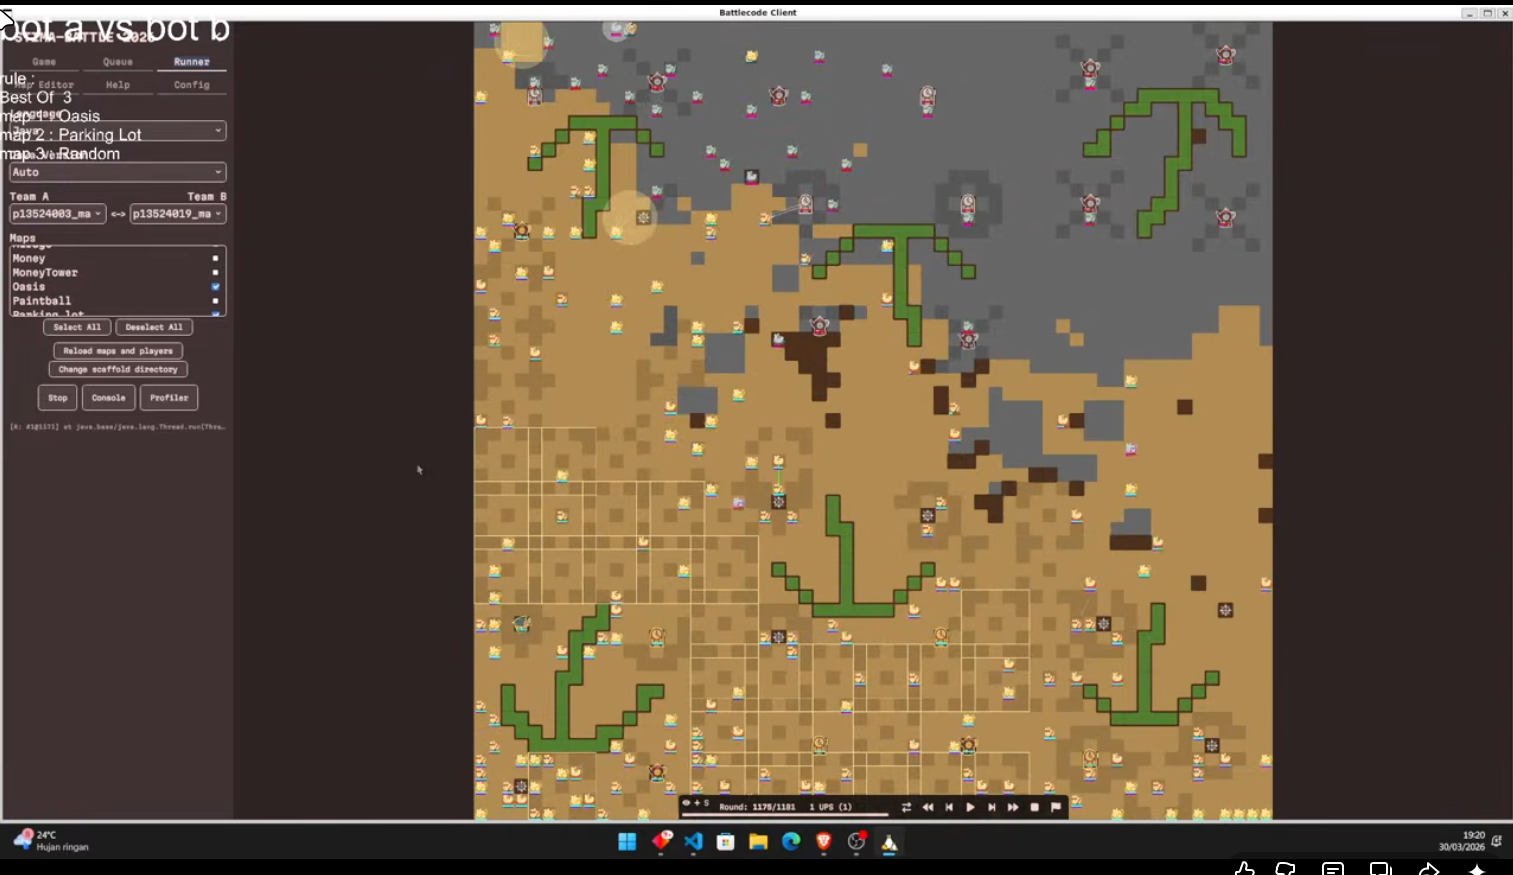
\includegraphics[width=\textwidth]{public/match1vs18224003/oasis.png}
        \caption{\textit{Oasis}}
    \end{subfigure}
    \hfill
    \begin{subfigure}[b]{0.48\textwidth}
        \centering
        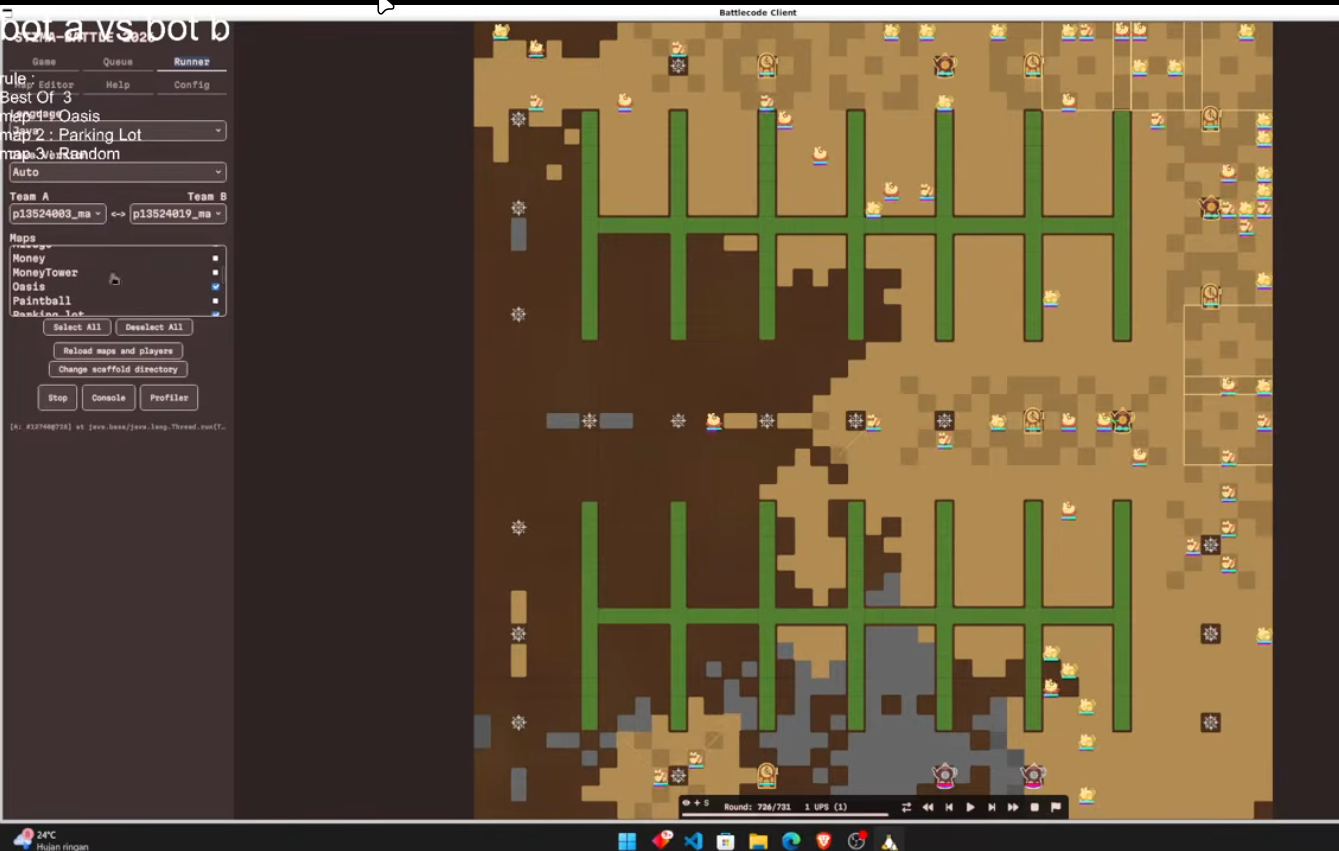
\includegraphics[width=\textwidth]{public/match1vs18224003/parking-lot.png}
        \caption{\textit{Parking Lot}}
    \end{subfigure}
    \caption{Pertandingan 1 vs 18224003 (Menang 2-0, Emas)}
\end{figure}

\begin{figure}[H]
    \centering
    \begin{subfigure}[b]{0.48\textwidth}
        \centering
        
\includegraphics[width=\textwidth]{public/match2vs13524113/oasis.png}
        \caption{\textit{Oasis}}
    \end{subfigure}
    \hfill
    \begin{subfigure}[b]{0.48\textwidth}
        \centering
        
\includegraphics[width=\textwidth]{public/match2vs13524113/parking-lot.png}
        \caption{\textit{Parking Lot}}
    \end{subfigure}
    \caption{Pertandingan 2 vs 13524113 (Menang 2-0, Emas)}
\end{figure}

\begin{figure}[H]
    \centering
    \begin{subfigure}[b]{0.48\textwidth}
        \centering
        
\includegraphics[width=\textwidth]{public/match3vs13524014/oasis.png}
        \caption{\textit{Oasis}}
    \end{subfigure}
    \hfill
    \begin{subfigure}[b]{0.48\textwidth}
        \centering
        
\includegraphics[width=\textwidth]{public/match3vs13524014/parking-lot.png}
        \caption{\textit{Parking Lot}}
    \end{subfigure}
    \caption{Pertandingan 3 vs 13524014 (Menang 2-0, Perak)}
\end{figure}

Peta \textit{Oasis} yang lebih terbuka menunjukkan dominasi cat emas dari sisi
kami secara visual, sedangkan \textit{Parking Lot} yang berstruktur grid sangat
cocok dengan pendekatan ekspansi menara kami karena reruntuhan tersebar secara
reguler dan mudah dijangkau Soldier.

Yang menarik adalah pertandingan ketiga, di mana kami bermain sebagai tim
\textbf{perak} (pemain kedua). Meski tidak memiliki keunggulan giliran pertama,
bot kami tetap berhasil menang 2-0 --- membuktikan bahwa strategi tidak terlalu
bergantung pada posisi awal. Pertandingan di \textit{Oasis} berlangsung lebih
lama hingga ronde 679, mengindikasikan lawan memiliki pertahanan yang lebih kuat,
namun ekspansi kami akhirnya tak terbendung.

\subsection*{Kekalahan di Perempat Final (vs 13524018)}

Perjalanan kami terhenti di pertandingan keempat melawan 13524018 dengan skor
1-2. Kami berhasil memenangkan \textit{Parking Lot} (67\% vs 1.4\%), namun
kalah di \textit{Oasis} (23.4\% vs 69.3\%) dan peta ketiga (10.2\% vs 67\%).

\begin{figure}[H]
    \centering
    \begin{subfigure}[b]{0.48\textwidth}
        \centering
        
\includegraphics[width=\textwidth]{public/match4vs13524018/oasis.png}
        \caption{\textit{Oasis}: kita 23.4\% vs lawan 69.3\% --- \textbf{Kalah}}
    \end{subfigure}
    \hfill
    \begin{subfigure}[b]{0.48\textwidth}
        \centering
        
\includegraphics[width=\textwidth]{public/match4vs13524018/parking-lot.png}
        \caption{\textit{Parking Lot}: kita 67\% vs lawan 1.4\% --- \textbf{Menang}}
    \end{subfigure}
    \caption{Pertandingan 4 vs 13524018 --- peta 1 dan 2}
\end{figure}

\begin{figure}[H]
    \centering
    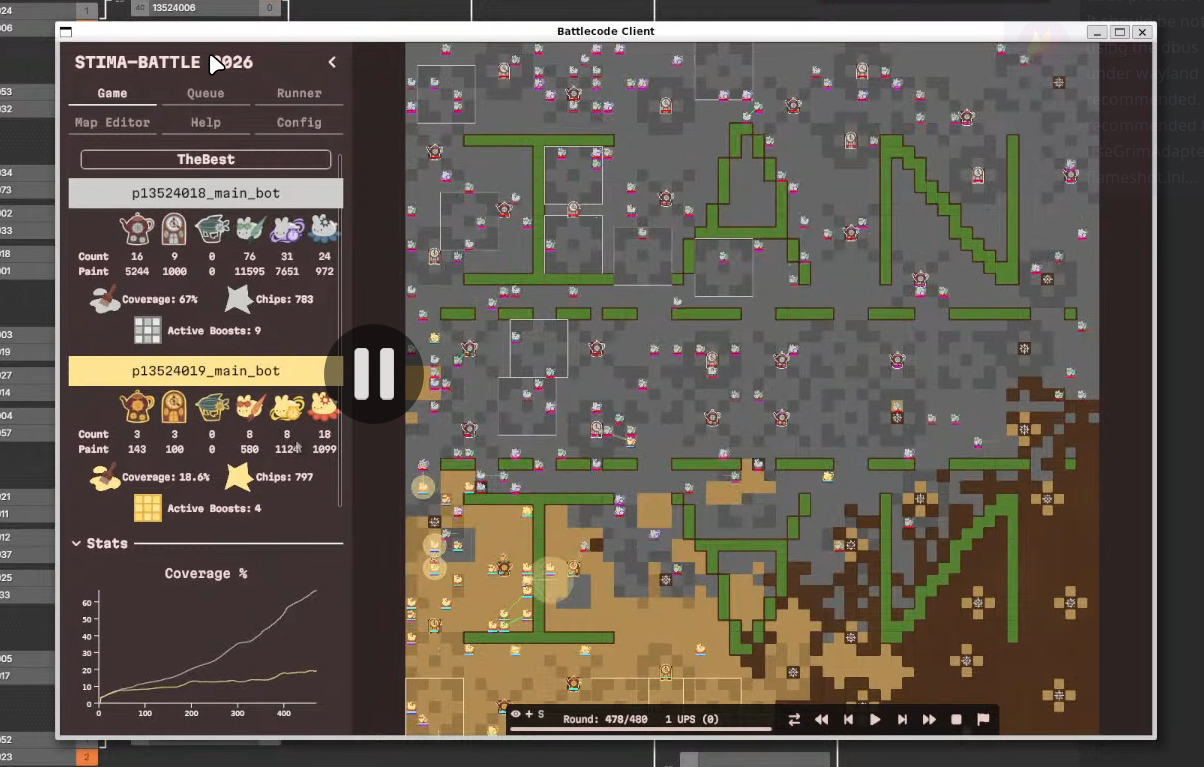
\includegraphics[width=0.65\textwidth]{public/match4vs13524018/map3.png}
    \caption{Pertandingan 4 vs 13524018 --- peta 3: kita 10.2\% vs lawan 67\% --- \textbf{Kalah}}
\end{figure}

Faktor penentu kekalahan di dua peta tersebut adalah perbedaan jumlah
\textit{active boosts} yang sangat mencolok: lawan memiliki 28 SRP aktif di
\textit{Oasis} dan 9 di peta ketiga, sementara kami hanya 4 di kedua peta.
Artinya lawan mendapatkan multiplikasi produksi sumber daya yang jauh lebih
besar, memungkinkan mereka mengecat lebih agresif di seluruh peta.

Ironisnya, kami justru memiliki 11.389 \textit{chips} yang tersisa saat kalah
di \textit{Oasis} --- surplus ekonomi yang tidak berhasil dikonversi menjadi
cakupan. Hal ini mengungkap dua kelemahan kritis:

\begin{enumerate}
    \item \textbf{Strategi SRP yang kurang agresif}: Bot baru membangun SRP
          setelah $\geq 3$ menara terbentuk, dan hanya di sekitar posisi Soldier
          saat itu. Tidak ada mekanisme untuk menyebarkan SRP secara sistematis
          ke seluruh peta sejak dini.
    \item \textbf{Surplus chips tidak terkonversi}: Ketika semua reruntuhan yang
          terjangkau sudah terbangun, bot tidak memiliki strategi alternatif untuk
          menghabiskan \textit{chips} secara produktif --- misalnya mempercepat
          \textit{upgrade} menara atau meningkatkan laju \textit{spawn}.
\end{enumerate}

% ================================================================
\section{Penutup}

\subsection{Ringkasan Pencapaian}

Bot \texttt{main\_bot} kelompok Jambi X Bekasi berhasil menembus \textbf{top 8}
turnamen STIMA-BATTLE 2026 dengan catatan 3 kemenangan 2-0 sebelum terhenti di
perempat final. Pencapaian ini membuktikan bahwa pendekatan greedy lokal dengan
kombinasi state machine, koordinasi multi-unit, dan sistem komunikasi sederhana
cukup kompetitif dalam arena turnamen nyata.

Kekuatan utama bot kami:
\begin{itemize}
    \item \textbf{Ekspansi menara yang konsisten}: Greedy decision pada SoldierBot
          secara efektif memprioritaskan pembangunan menara, menghasilkan jaringan
          yang kuat dalam fase awal.
    \item \textbf{Fleksibilitas komposisi unit}: Fase-based spawning pada TowerBot
          memastikan keseimbangan antara ekspansi (Soldier), cakupan (Splasher), dan
          pertahanan (Mopper).
    \item \textbf{Navigasi yang robust}: Kombinasi FuzzyMove dan BugNav dengan
          anti-osilasi ring buffer mencegah unit terjebak dan memastikan jangkauan
          ke seluruh peta.
    \item \textbf{Robustness terhadap posisi}: Bot terbukti efektif baik sebagai
          tim emas maupun perak (kemenangan di Babak 3 sebagai tim perak).
\end{itemize}

\subsection{Pelajaran dan Perbaikan yang Disarankan}

Berdasarkan kekalahan di babak 4, beberapa perbaikan yang dapat dilakukan:

\begin{enumerate}
    \item \textbf{Strategi SRP yang lebih agresif}: Membangun SRP lebih awal
          (mulai dari menara pertama) dan menyebarkan pusat SRP ke seluruh peta
          menggunakan \textit{modulo 4 trick} secara sistematis --- bukan hanya di
          sekitar posisi Soldier saat itu.
    \item \textbf{Pemanfaatan surplus chips}: Menambahkan logika untuk meng-upgrade
          menara secara lebih agresif atau meningkatkan laju spawn unit saat
          \textit{chips} sangat berlimpah.
    \item \textbf{Eksplorasi terpetakan}: Mengimplementasikan pembagian sektor peta
          antar-Soldier untuk memastikan seluruh reruntuhan tereksplor, sehingga
          tidak ada reruntuhan yang terbengkalai karena semua Soldier menuju lokasi
          yang sama.
    \item \textbf{Koordinasi SRP antar-unit}: Menggunakan sistem pesan untuk
          membagi tanggung jawab SRP antar-Soldier, menghindari redundansi saat
          dua Soldier mencoba membangun SRP di lokasi yang sama.
\end{enumerate}

\subsection{Refleksi}

Pengalaman mengikuti STIMA-BATTLE 2026 memberikan wawasan mendalam tentang
penerapan algoritma greedy dalam lingkungan multi-agent yang kompetitif. Desain
berbasis greedy lokal terbukti sederhana untuk diimplementasi dan di-debug, namun
memiliki keterbatasan inheren: tanpa koordinasi global, bot sulit mencapai
distribusi SRP yang optimal di seluruh peta.

Ke depannya, pendekatan yang lebih canggih seperti koordinasi berbasis
\textit{shared memory} (melalui sistem pesan yang lebih kaya), atau bahkan strategi
berbasis \textit{dynamic programming} untuk alokasi unit, dapat meningkatkan
performa secara signifikan --- terutama pada aspek SRP farming yang terbukti krusial
dalam menentukan hasil pertandingan di level yang lebih tinggi.

\end{document}
